\documentclass{article}

\usepackage{arxiv}

\usepackage[utf8]{inputenc} % allow utf-8 input
\usepackage[T1]{fontenc}    % use 8-bit T1 fonts
\usepackage{hyperref}       % hyperlinks
\hypersetup{hidelinks = true}
\usepackage{url}            % simple URL typesetting
\usepackage{booktabs}       % professional-quality tables
\usepackage{amsfonts}       % blackboard math symbols
\usepackage{amsmath}
\usepackage{amssymb}
\usepackage{nicefrac}       % compact symbols for 1/2, etc.
\usepackage{microtype}      % microtypography
\usepackage{minted}

\usepackage{fancyvrb}
\usepackage{mathtools}
\DeclarePairedDelimiter{\ceil}{\lceil}{\rceil}

\usepackage{graphicx}
\usepackage{subcaption}

% ENVIRONMENTS
\usepackage{amsthm}
\theoremstyle{plain}
\newtheorem{definition}{Definition}[section]
\newtheorem{lemma}[definition]{Lemma}
\newtheorem{proposition}[definition]{Proposition}
\newtheorem{corollary}[definition]{Corollary}
\newtheorem{example}[definition]{Example}
\theoremstyle{remark}
\newtheorem{remark}[definition]{Remark}

% TEXT-MODE MACROS
\newcommand{\IN}{\mathbb{N}}
\newcommand{\IR}{\mathbb{R}}
\newcommand{\IZ}{\mathbb{Z}}
\newcommand{\union}{\cup}
\newcommand{\Union}{\bigcup}
\newcommand{\code}{\texttt} % for use as \code{test()}
\newcommand{\defn}{\emph} % for use as \defn{...}

% MATH-MODE MACROS
\newcommand{\qtext}[1]{\quad\text{#1}\quad} % for use as \def{...} inside text
\newcommand{\ra}{\rightarrow}
\newcommand{\lra}{\longrightarrow}
\newcommand{\floor}[1]{\lfloor#1\rfloor}
\newcommand{\abs}[1]{|#1|}
\newcommand{\eps}{\epsilon}


\title{circllhist}

\subtitle{The Circonus Log-Linear Histogram}

\author{
  Heinrich Hartmann \\
  \texttt{heinrich.hartmann@circonus.com} \\
  Circonus \\
  \And
  Theo Schlossnagle \\
  \texttt{theo.schlossnagle@circonus.com} \\
  Circonus
}

\begin{document}

\maketitle

\begin{abstract}
  The circllhist histogram is a simple, fast and memory efficient data structure for capturing
  and processing large number of samples, that is particularly suited for applications in
  IT infrastructure monitoring.

  The circllhist allows arbitrary merging of pre-aggregated data without additional loss of accuracy,
  and the approximation of percentiles with low expected error and a-priori bounded maximal error.

  Open-source implementations are available for C/lua/python/Go/Java/JavaScript.
\end{abstract}

\tableofcontents

\input{part1.tex}

\clearpage
\section{Theory}

\begin{figure}
  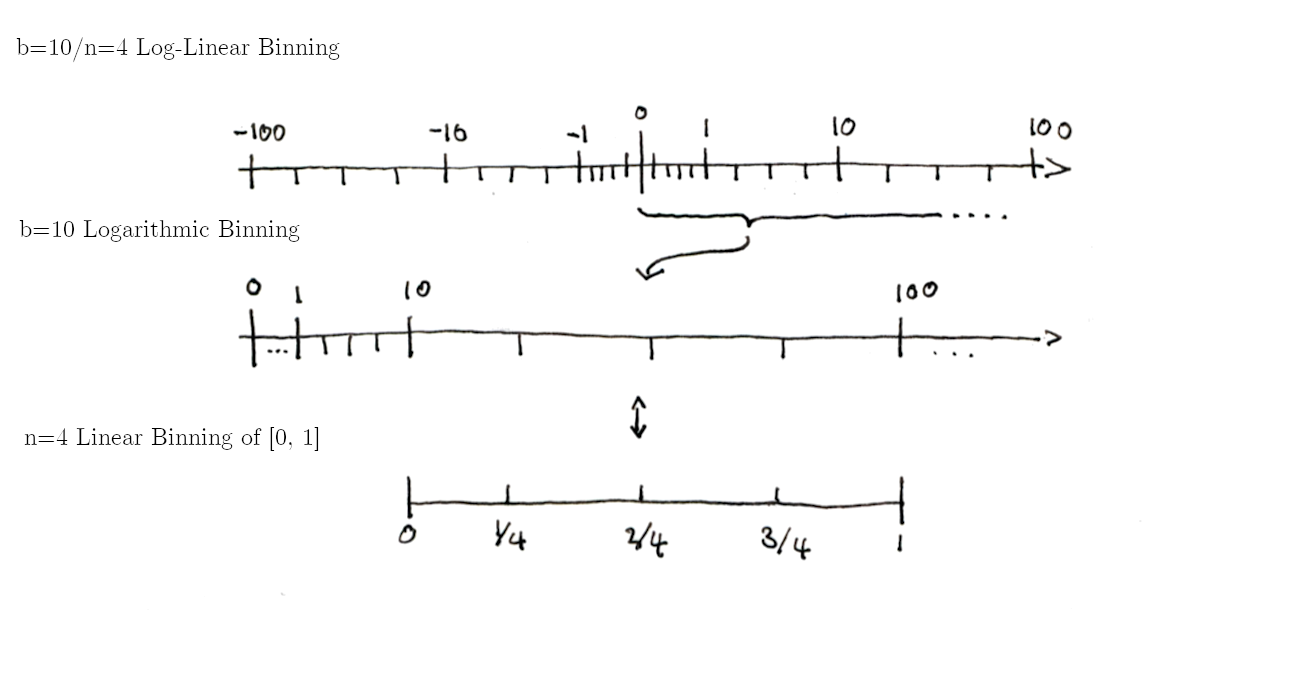
\includegraphics[width=\textwidth]{assets/LLBins.png}
  \caption{Construction of the Log-Linear Binning}
  \label{fig:llbins}
\end{figure}

The idea behind the circllhist is illustrated in Figure \ref{fig:llbins}, and quick to explain.
We start with a logarithmic binning of the real axes, that has bins at the powers of ten.
\begin{center}
  \begin{BVerbatim}
    ... 0.01, 0.1, 1, 10, 100, ...
  \end{BVerbatim}
\end{center}
We divide each logarithmic bin into $n=90$ equally spaced segments. In this way the bin boundaries
are preciesly the base-10, precision-2 floating point numbers:
\begin{center}
\begin{BVerbatim}
... 1.0,  1.1,  1.2,  ...   9.9,
     10,   11,   12,  ...    99,
    100,  110,  120,  ...   990, ...
\end{BVerbatim}
\end{center}
Those are the bin boundaries for the circllhist data structure.
When samples are inserted into the circllhist, we retain counts of the number of samples in each bin.
This information allows us to approximate the original location of the inserted samples with a
maximal relative error less than $5\%$.

In this section we develop an abstract theory of histograms to a degree that allows us to
formally define circllhist as a linear refinement of a logarithmic histogram structure,
and derive basic properties and error bounds.

\subsection{Binnings}

\begin{definition}
  Let $D \subset \IR$ be a connected subset of the real axes (e.g. $D=\IR, D=[0,1)$).
  A binning of $D$ is a collection of intervals $Bin[i], i \in I$, that are disjoint and collectively cover the binning domain $D$:
  \begin{align*}
    D = \Union_{i\in I} Bin[i] \qtext{and} Bin[i] \cap Bin[j] = \emptyset \qtext{for} i \neq j.
  \end{align*}
  The map that associates to each $x \in D$ the unique index $i$ so that $x \in Bin[i]$ is called
  binning map and is denoted as $bin(x) = i$.
\end{definition}

\begin{remark}
  The binning map $bin: D \ra I$ determines the binning via $Bin[i] = \{ x \in D \,|\, bin(x) = i \}$.
\end{remark}

\begin{example}
  The linear binning of $\IR$ is given by $I = \IZ$, with
  \begin{align*}
    Bin[i] = [i, i+1)  \qtext{and} bin(x)=\floor{x}
  \end{align*}
\end{example}

\begin{example}
  The length $n$ linear binning of $[0,1)$ is given by $I = \{0, \dots, n-1\}$, with
    \begin{align*}
      Bin^{Lin}_n[i]   = [ \frac{i}{n}, \frac{i+1}{n} )
      \qtext{and}
      bin^{Lin}_n(x) = \floor{x \cdot n}
    \end{align*}
\end{example}

\begin{example}
  The logarithmic binning with basis $b > 0$ of $\IR_{>0}$ is given by $I=\IZ$, with
  \begin{align*}
    Bin^{Log}_b[i] = [b^i, b^{i+1})
    \qtext{and}
    bin^{Log}_b(x)=\floor{\log_b(x)}
  \end{align*}
\end{example}

\begin{definition}\label{ref}
  Given a map $\alpha: I \ra J$, and a binning $(I, Bin)$, we can define a new binning
  $(J, Bin^*)$ by setting:
  \begin{align*}
    Bin^*[j] = \Union_{i, \alpha(i) = j} Bin[i], \qtext{and} bin^*(x) = \alpha(bin(x))
  \end{align*}
  In this situation we call $(J, Bin^*)$ a coarsening of $(I, Bin)$, and $(I, Bin)$ a refinement of $(J, Bin^*)$.
\end{definition}

\begin{definition}\label{lref}
  Given a binning $Bin[i], i\in I$ with half-open bins $Bin[i] = [a_i, b_i)$.
  The length-n linear refinement of $(I, Bin)$, is given by the index set $I \times \{0,\dots, n-1\}$,
  bins
  \begin{align*}
    L_nBin[i,j] = [ a_i + \frac{j}{n}(b_i - a_i), a_i + \frac{j+1}{n}(b_i - a_i) )
  \end{align*}
  and binning map
  \begin{align*}
    L_nbin(x) = ( bin(x), \floor{\frac{x - a_{bin(x)}}{b_{bin(x)} - a_{bin(x)}} \cdot n } ).
  \end{align*}
\end{definition}

\begin{proof}
  To verify the binning map we have to show that $x \in L_nBin[ L_nbin(x) ]$ for all $x \in D$.
  Let $(i,j) = L_nbin(x)$.
  Since $i = bin(x)$, we know that $x \in [a_i, b_i)$.
  Now we consider the linear map $\phi(x) = (x-a_i)/(b_i-a_i)$ which maps $Bin[i]$ bijectively to $[0,1)$.
  We have $j = \floor{ n \phi(x) }$ by definition of $L_nbin(x)$.
  To show that $x \in L_nBin[ L_nbin(x) ]$ it suffices to verify
  that $\phi(x) \in \phi(L_nBin[i,j]) = [ \frac{j}{n}, \frac{j+1}{n} )$.
  And indeed,
  \begin{align*}
    \frac{j}{n} = \frac{\floor{ n \phi(x) }}{n} \leq \phi(x)
    \leq \frac{\ceil{n \phi(x)}}{n} < \frac{\floor{ n \phi(x) } + 1 }{n} =  \frac{j+1}{n}
  \end{align*}
\end{proof}

\begin{lemma}
  The length-n linear refinement of a binning $(I, Bin)$ is a refinement in the sense of Definition \ref{ref}.
  The index map is given by $\alpha(i,j) = i$ for $i \in I$, $j \in \{0,\dots,n-1\}$.
\end{lemma}

\begin{proof}
  We have to show that $\Union_{j} L_nBin[i,j] = Bin[i]$, for all $i \in I$.
  Again we consider the linear bijection $\phi(x) = (x-a_i)/(b_i-a_i)$, which maps $Bin[i]$ to $[0,1)$ and $L_nBin[i,j]$ to $[j/n, (j+1)/n)$.
  Hence it suffices to show that $[j/n, (j+1)/n)$ cover $[0,1)$ for $j=0,\dots,n$ which is evident.
\end{proof}

\subsection{Log-Linear Binnings}

\subsection{Histogram Operations}

\subsection{Merging}

\subsection{Percentiles}

\section{Implementation}

\section{Evaluation}

\clearpage
\subsection{Calibration}

\begin{figure}
   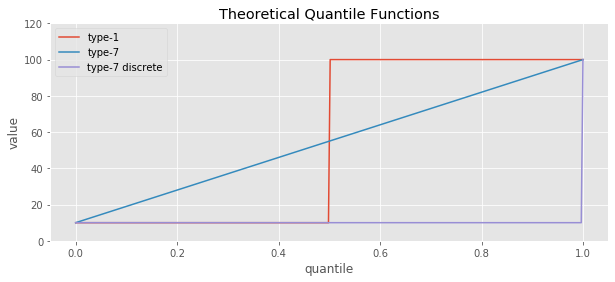
\includegraphics[width=\textwidth]{evaluation/images/quantile_comparison.png}
   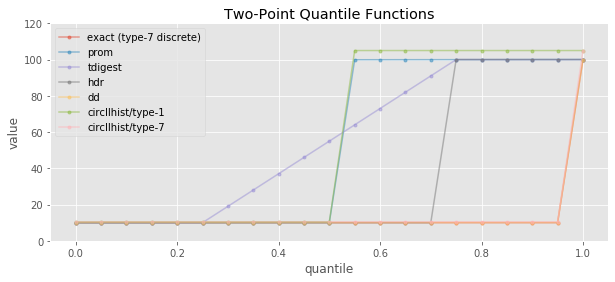
\includegraphics[width=\textwidth]{evaluation/images/Two_Points_quantile_comparison.png}
   \caption{Percentile functions on two-point dataset}
\end{figure}

\begin{figure}
  \centering
  \begin{tabular}{lrrrrrrr}
\toprule
{} &   exact &    prom &  tdigest &     hdr &      dd &  circllhist/type-1 &  circllhist/type-7 \\
\midrule
q0  &  10.000 &   9.900 &   10.000 &   9.999 &  10.000 &             10.500 &             10.500 \\
q.1 &  10.000 &   9.930 &   10.000 &  10.006 &  10.075 &             10.500 &             10.500 \\
q.2 &  10.000 &   9.960 &   10.000 &  10.006 &  10.075 &             10.500 &             10.500 \\
q.3 &  10.000 &   9.990 &   19.000 &  10.006 &  10.075 &             10.500 &             10.500 \\
q.4 &  10.000 &  10.020 &   37.000 &  10.006 &  10.075 &             10.500 &             10.500 \\
q.5 &  10.000 &  10.050 &   55.000 &  10.006 &  10.075 &             10.500 &             10.500 \\
q.6 &  10.000 &  99.930 &   73.000 &  10.006 &  10.075 &            105.000 &             10.500 \\
q.7 &  10.000 &  99.960 &   91.000 &  10.006 &  10.075 &            105.000 &             10.500 \\
q.8 &  10.000 &  99.990 &  100.000 & 100.019 &  10.075 &            105.000 &             10.500 \\
q.9 &  10.000 & 100.020 &  100.000 & 100.019 &  10.075 &            105.000 &             10.500 \\
q1  & 100.000 & 100.050 &  100.000 & 100.019 & 100.000 &            105.000 &            105.000 \\
\bottomrule
\end{tabular}

  \caption{Percentile values of the two-point dataset $[10,100]$}
\end{figure}

\clearpage
\subsection{Datasets}

\begin{figure}
   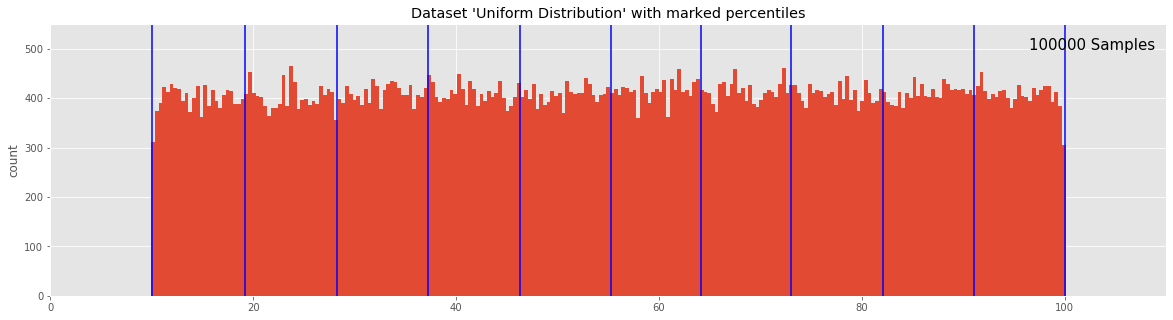
\includegraphics[width=\textwidth]{evaluation/images/Uniform_Distribution_distribution_percentiles.png}
   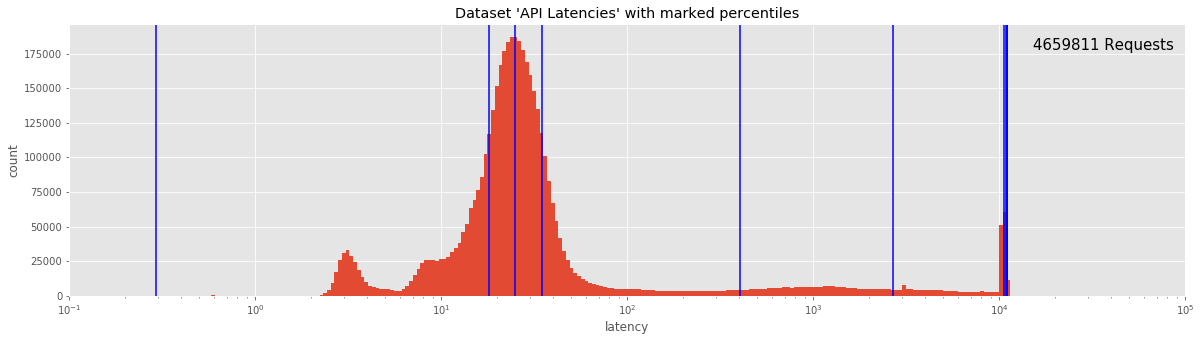
\includegraphics[width=\textwidth]{evaluation/images/API_Latencies_distribution_percentiles.png}
   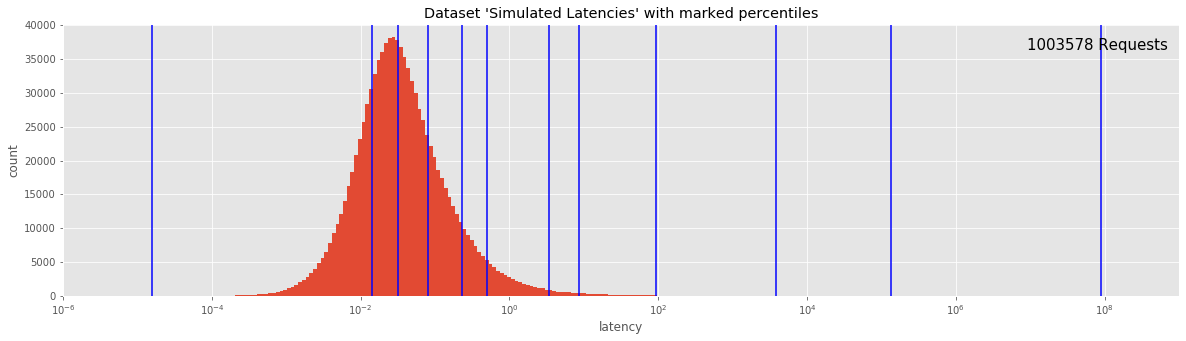
\includegraphics[width=\textwidth]{evaluation/images/Simulated_Latencies_distribution_percentiles.png}
   \caption{Datasets}
\end{figure}

\clearpage
\subsection{Size}

\begin{figure*}[t!]
  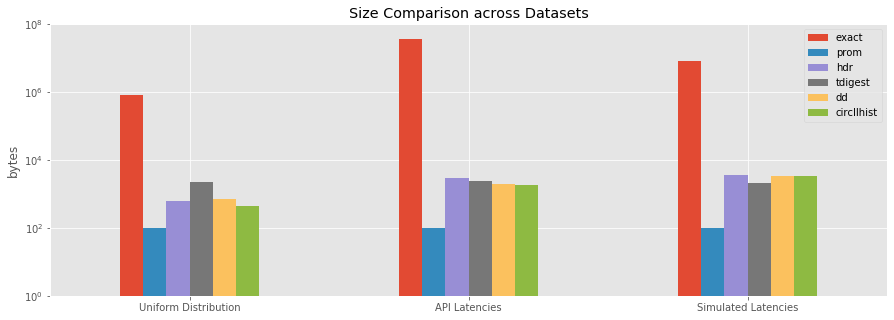
\includegraphics[width=\textwidth]{evaluation/images/all_size.png}
  \caption{Size Comparison}
\end{figure*}

\begin{figure}
  \centering
  \begin{tabular}{lrrrrrr}
\toprule
{} &     exact &  prom &  hdr &  tdigest &    dd &  circllhist \\
\midrule
Uniform Distribution &    800000 &    96 &  621 &     2224 &   716 &         453 \\
API Latencies        &  37278488 &    96 & 2994 &     2368 &  1902 &        1866 \\
Simulated Latencies  &   8028624 &    96 & 3699 &     2096 &  3428 &        3396 \\
\bottomrule
\end{tabular}

  \caption{Aggregation sizes in kb}
\end{figure}

\clearpage
\subsection{Performance}

\begin{figure}
  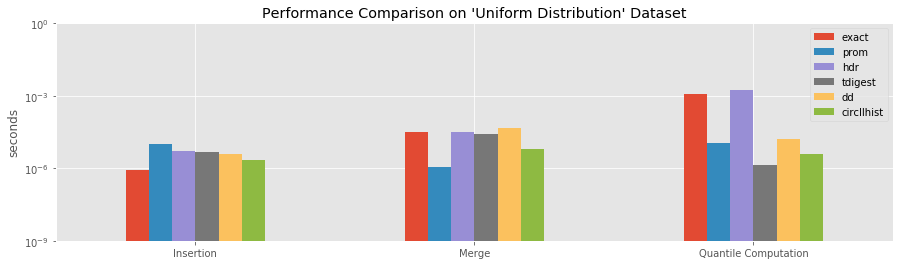
\includegraphics[width=\textwidth]{evaluation/images/Uniform_Distribution_perf.png}
  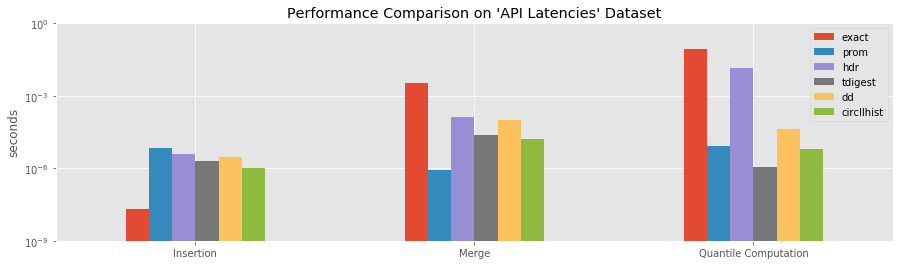
\includegraphics[width=\textwidth]{evaluation/images/API_Latencies_perf.png}
  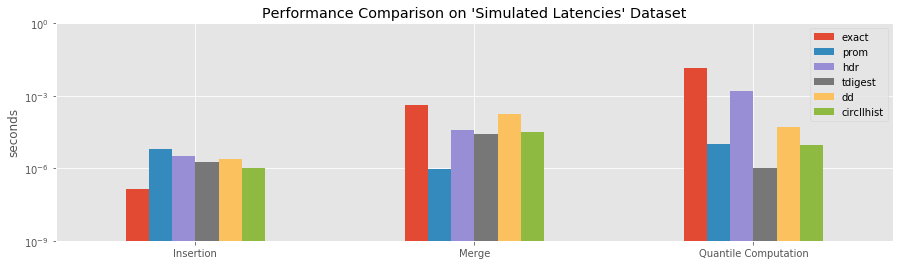
\includegraphics[width=\textwidth]{evaluation/images/Simulated_Latencies_perf.png}
  \caption{Performance Comparison}
\end{figure}

Tables in usec

Uniform\\
\begin{tabular}{lrrrrrr}
\toprule
{} &  exact &  prom &    hdr &  tdigest &   dd &  circllhist \\
\midrule
Insertion            &    0.9 &  10.5 &    7.7 &      4.6 &  3.8 &         2.2 \\
Merge                &   33.1 &   1.1 &  129.0 &     26.9 & 45.8 &         6.3 \\
Quantile Computation & 1180.3 &  11.3 & 9684.9 &      1.4 & 17.1 &         3.8 \\
\bottomrule
\end{tabular}


API Latencies\\
\begin{tabular}{lrrrrrr}
\toprule
{} &   exact &  prom &    hdr &  tdigest &    dd &  circllhist \\
\midrule
Insertion            &     0.0 &   6.9 &    3.7 &      2.0 &   3.0 &         1.0 \\
Merge                &  3487.6 &   0.9 &   34.1 &     24.0 & 104.6 &        16.1 \\
Quantile Computation & 83773.2 &   8.3 & 1931.4 &      1.1 &  42.6 &         6.1 \\
\bottomrule
\end{tabular}


Simulated API Latency Data\\
\begin{tabular}{lrrrrrr}
\toprule
{} &   exact &  prom &     hdr &  tdigest &    dd &  circllhist \\
\midrule
Insertion            &     0.1 &   6.5 &     3.5 &      1.9 &   2.5 &         1.0 \\
Merge                &   415.4 &   1.0 &   135.6 &     27.1 & 185.7 &        31.7 \\
Quantile Computation & 14222.5 &  10.0 & 11198.1 &      1.1 &  51.4 &         8.9 \\
\bottomrule
\end{tabular}


\clearpage
\subsection{Accuracy}

\begin{figure}
  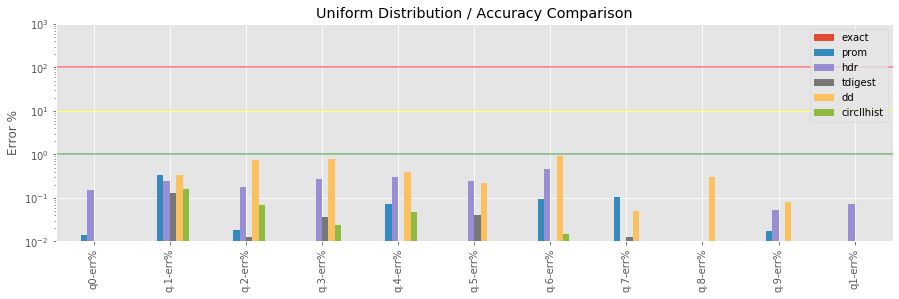
\includegraphics[width=\textwidth]{evaluation/images/Uniform_Distribution_accuracy.png}
  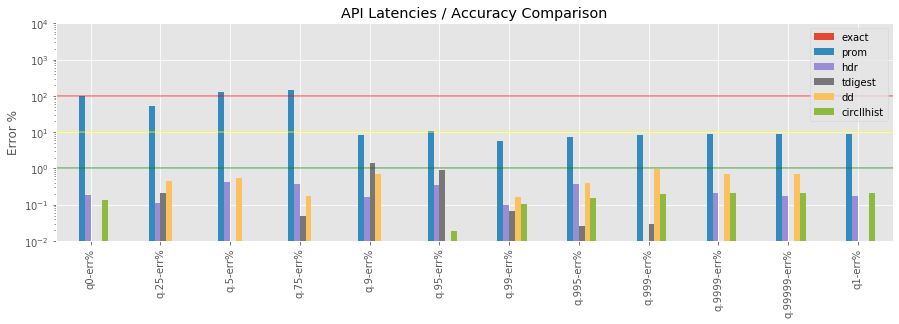
\includegraphics[width=\textwidth]{evaluation/images/API_Latencies_accuracy.png}
  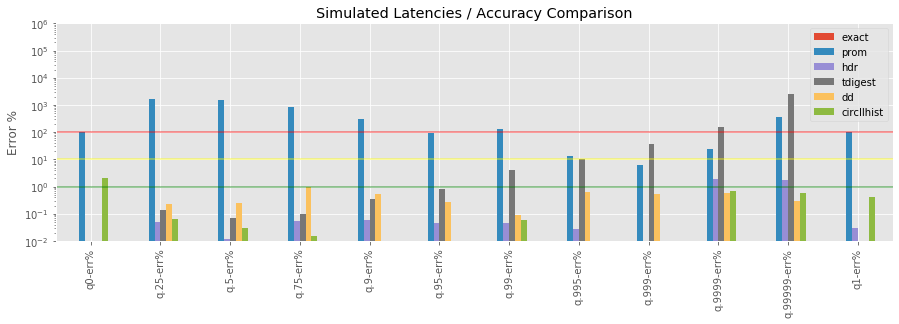
\includegraphics[width=\textwidth]{evaluation/images/Simulated_Latencies_accuracy.png}
  \caption{Accuracy Comparison}
\end{figure}

\begin{figure}
  Uniform\\
  \begin{tabular}{lrrrrr}
\toprule
{} &  prom &   hdr &  tdigest &    dd &  circllhist \\
\midrule
q0-err\%  & 0.014 & 0.156 &    0.000 & 0.000 &       0.005 \\
q.1-err\% & 0.339 & 0.248 &    0.129 & 0.342 &       0.160 \\
q.2-err\% & 0.018 & 0.178 &    0.013 & 0.736 &       0.069 \\
q.3-err\% & 0.006 & 0.273 &    0.036 & 0.794 &       0.024 \\
q.4-err\% & 0.074 & 0.297 &    0.003 & 0.394 &       0.048 \\
q.5-err\% & 0.000 & 0.243 &    0.040 & 0.216 &       0.007 \\
q.6-err\% & 0.094 & 0.468 &    0.006 & 0.931 &       0.015 \\
q.7-err\% & 0.105 & 0.006 &    0.013 & 0.050 &       0.000 \\
q.8-err\% & 0.004 & 0.010 &    0.001 & 0.307 &       0.009 \\
q.9-err\% & 0.017 & 0.053 &    0.006 & 0.081 &       0.000 \\
q1-err\%  & 0.000 & 0.073 &    0.000 & 0.000 &       0.001 \\
\bottomrule
\end{tabular}

  API Latencies\\
  \begin{tabular}{lrrrrr}
\toprule
{} &    prom &   hdr &  tdigest &    dd &  circllhist \\
\midrule
q0-err\%      & 100.000 & 0.038 &    0.000 & 0.000 &       0.134 \\
q.25-err\%    &  52.671 & 0.035 &    0.216 & 0.460 &       0.000 \\
q.5-err\%     & 126.469 & 0.038 &    0.000 & 0.538 &       0.003 \\
q.75-err\%    & 145.163 & 0.061 &    0.049 & 0.171 &       0.001 \\
q.9-err\%     &   8.230 & 0.007 &    1.382 & 0.685 &       0.006 \\
q.95-err\%    &  10.636 & 0.023 &    0.907 & 0.006 &       0.019 \\
q.99-err\%    &   5.662 & 0.031 &    0.066 & 0.164 &       0.105 \\
q.995-err\%   &   7.313 & 0.064 &    0.026 & 0.399 &       0.155 \\
q.999-err\%   &   8.584 & 0.010 &    0.030 & 0.979 &       0.202 \\
q.9999-err\%  &   8.862 & 0.019 &    0.007 & 0.715 &       0.216 \\
q.99999-err\% &   8.891 & 0.050 &    0.003 & 0.683 &       0.216 \\
q1-err\%      &   8.894 & 0.047 &    0.000 & 0.000 &       0.217 \\
\bottomrule
\end{tabular}

  Simulated API Latency Data\\
  \begin{tabular}{lrrrrr}
\toprule
{} &     prom &   hdr &  tdigest &    dd &  circllhist \\
\midrule
q0-err\%      &  100.000 & 0.407 &    0.000 & 0.000 &       2.110 \\
q.25-err\%    & 1706.372 & 0.232 &    0.141 & 0.238 &       0.062 \\
q.5-err\%     & 1523.356 & 0.012 &    0.069 & 0.243 &       0.029 \\
q.75-err\%    &  857.929 & 0.054 &    0.101 & 0.957 &       0.016 \\
q.9-err\%     &  296.620 & 0.689 &    0.342 & 0.546 &       0.009 \\
q.95-err\%    &   95.263 & 0.632 &    0.813 & 0.277 &       0.004 \\
q.99-err\%    &  133.561 & 0.146 &    4.152 & 0.087 &       0.059 \\
q.995-err\%   &   13.454 & 0.029 &   10.259 & 0.649 &       0.008 \\
q.999-err\%   &    6.136 & 0.406 &   36.221 & 0.519 &       0.002 \\
q.9999-err\%  &   23.154 & 1.933 &  149.000 & 0.599 &       0.670 \\
q.99999-err\% &  355.293 & 2.224 & 2559.294 & 0.301 &       0.570 \\
q1-err\%      &   98.875 & 0.347 &    0.000 & 0.000 &       0.409 \\
\bottomrule
\end{tabular}

\end{figure}

\bibliographystyle{unsrt}
\begin{thebibliography}{1}

\bibitem{tdigest}
T. Dunning and O. Ertl.
\newblock  Computing extremeley accurate quantiles using t-digests.
\newblock \url{https://github.com/tdunning/t-digest}, 2017.

\bibitem{dd}
M. Charles, J.E. Rim, H.K. Lee.
\newblock DDSketch: A fast and fully-mergeable quantile sketch with relative-error guarantees.
\newblock Proceedings of the VLDB Endowment 12.12 (2019): 2195-2205.

\bibitem{hdr}
G. Tene,
\newblock HdrHistogram: A high dynamic range (hdr) histogram
\newblock \url{http://hdrhistogram.org/}, 2012

\bibitem{libcircllhist}
  Circonus,
  \newblock libcircllhist: An implementation of Circonus Log-Linear Histograms
  \newblock \url{https://github.com/circonus-labs/libcircllhist}, 2016

\end{thebibliography}
\end{document}
